\genHeader
\label{chap:Learning-Box-to-Dictionary-and-Back-Again}

\requiredTime{1h 30min}

If you're just joining us in this part and are only interested in bidirectional model transformations with \emph{Triple Graph Grammars} then welcome! To ensure
eMoflon is running correctly however, you should at least work through Part I for the required installation and setup instructions. We try to assume as little
as possible from the previous parts in the handbook series, and give appropriate references where necessary.

To briefly review what we have done so far: we have developed Leitner's learning box by specifying its \emph{abstract syntax} and \emph{static semantics} as a
\emph{metamodel}, and finally implementing its \emph{dynamic semantics} via Story Driven Modeling (programmed graph transformations). If the previous sentence
could just as well have been in Chinese\footnote{Replace with Greek if you are chinese.  If you are chinese but speak fluent Greek, then we give up. You get the
point anyway, right?} for you, then please work through Parts II and III.

Even though SDMs are crazily cool (don't you forget that!), it is rather unsatisfactory implementing a \emph{bidirectional} transformation as two unidirectional
transformations. If you critically consider the straighforward solution of specifying forward and backward transformations as separate SDMs, you should be able
to realise the following problems.

\vspace{-0.5cm}

\begin{description}
\item[Productivity:] We have to implement two transformations that are really quite similar, \emph{separately}. This simply doesn't feel productive.
Wouldn't it be nice to implement one direction such as the forward transformation, then get the backward transformation for free? How about deriving
forward \emph{and} backward transformations from a common joint specification?

\item[Maintainability:] Another maybe even more important point is that two separate transformations often become a pain to maintain and keep
\emph{consistent}. If the forward transformation is ever adjusted to produce a different target structure, the backward transformation must be updated
appropriately to accommodate the change, and vice-versa.  Again, it would be great if the language offered some support.

\item[Traceability:] Finally, one often needs to identify the reason why a certain object has been created during a transformation process. This increases the
trust in the specified transformation and is essential for working with systems that may actually do some harm (i.e., automotive or medical systems). With two
separate transformations, \emph{traceability} has to be supported manually! Traceability links can also be used to propagate changes made to an existing pair of
models \emph{incrementally}, i.e., without recreating the models from scratch. This is not only more efficient in most cases, but is also sometimes necessary to
avoid losing information in one model that simply cannot be recreated with the other model.
\end{description}

Our goal is to investigate how Triple Graph Grammars (TGGs), a \emph{bidirectional} transformation language, can be used to address these problems. To
continue with our running example, we plan to transform \texttt{Leit\-ners\-Learn\-ing\-Box}, a partitioned container populated with unsorted cards that are
moved through the box as they are memorized,\footnote{For a detailed review on Leitner's Learning Box, see Part II, Section 1} into a \texttt{Dictionary}, a
single flat container able to hold an unlimited number of entries classified by difficulty (Fig.~\ref{fig:transformIdea}).

\vspace{0.5cm}

\begin{figure}[htbp]
\begin{center}
  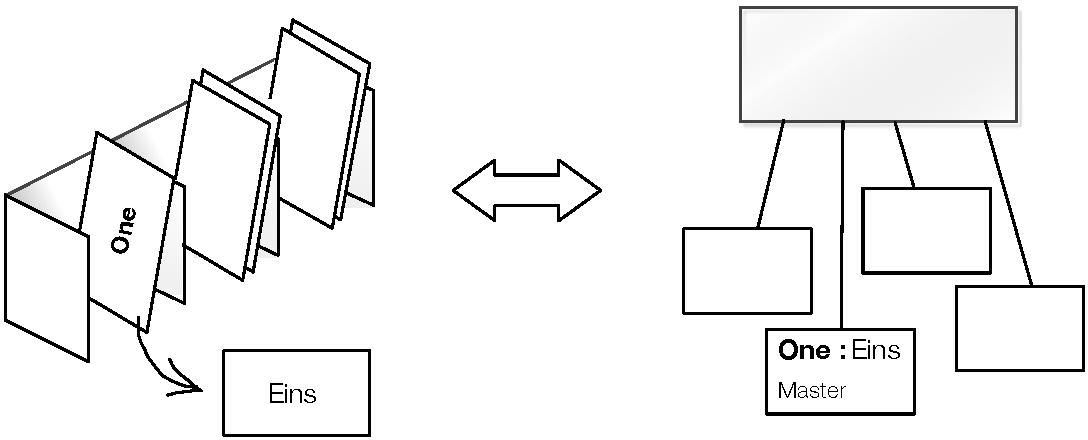
\includegraphics[width=\textwidth]{TGGTransformationExample.pdf}
  \caption{Transforming Leitner's learning box into a dictionary}
  \label{fig:transformIdea}
\end{center}
\end{figure}

\newpage

To briefly explain, each card in the box has a keyword on one side that a user can see, paired with a definition hidden on the opposite side. We will combine
each of these to create the keyword and content of a single dictionary entry, perhaps assigning a difficulty level based on the card's current position in the
box. We also want to be able to transform in the opposite direction, transforming each entry into a card by splitting up the contents, and inserting the new
element into a specific partition in the box. After a short introduction to TGGs and setting up your workspace correctly, we will see how to develop
your first bidirectional transformation!

